\section{Newtonsche Mechanik}
Um die Anwendung der Langrange-Mechanik zu verstehen, schauen wir uns zunächst
die Herleitung des einfachen mathematischen Pendels mittels Newtonscher-Mechanik an.
Im Fokus stehen dabei die Kräfte, die in einem System wirken.
Diese Kräfte haben zur Folge, dass eine Masse \(m\) beschleunigt wird.
Die Bewegungsgleichung wird bestimmt durch die Überlagerung aller Kräfte, die auf
die Masse wirken.

\subsection{Bewegungsgleichung einfaches Pendel}
Am Beispiel des einfachen Pendels sieht dies folgendermassen aus
(siehe Abbildung \ref{fig:pendulum1}).
Man hat drei Kräfte, die auf das Pendel wirken.
Ganz grundlegend die Gewichtskraft \(F_g\) und durch die Befestigung der Masse
an einem Stab folgen die Kräfte \(F_t\) mit \(F_r\).
Dabei ist \(F_r\) die Zwangskraft, welche die Masse auf dem Kreis um
den Aufhängepunkt hält.
Die Pendelmasse folgt der Kraft \(F_t\) und \(F_r\) ist die Kraft, welche
das Pendel auf den Stab oder Seil ausübt.

\begin{figure}
    \centering
    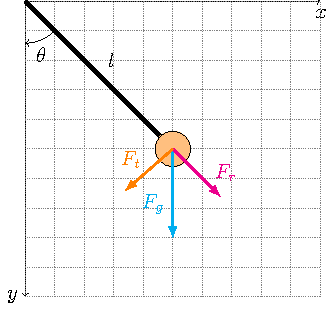
\includegraphics{papers/doppelpendel/images/pendel_pic1.pdf}
    \caption{mathematisches Pendel}
    \label{fig:pendulum1}
\end{figure}

Wir wissen, dass gemäss zweitem Newtonschen Gesetz
\begin{align*}
    F &= ma
\end{align*}
gilt. Wenden wir dies auf unser Problem an, erhalten wir
\begin{align*}
    F_t &= m l \ddot{\theta}.
\end{align*}
Nun betrachten wir das Ganze aus geometrischer Sicht und
lesen aus Abbildung \ref{fig:pendulum1}
\begin{align*}
    F_t &= F_g \sin(\theta)
    \shortintertext{ab. Umformuliert ergibt das}
    F_t &= -m g \sin(\theta).
    \shortintertext{Setzen wir alles gleich, dann erhalten wir}
    m l \ddot{\theta} &= -m g \sin(\theta).
\end{align*}
Aufgelöst nach der Beschleunigung resultiert daraus
\begin{align}
        \label{eq:mathematisches_pendel}
        \ddot{\theta} &= -\frac{g}{l} \sin(\theta).
\end{align}
Damit ist die Gleichung des mathematischen Pendels hergeleitet.

\subsection{Vorteile der Lagrange Methode}
In diesem Fall könnten wir auch nach der Position \(\theta\) des Pendels auflösen,
aber wir geben uns hiermit schon zufrieden.
Wir stellen fest, dass wenn wenige Kräfte wirken und alle davon bekannt sind,
dann lässt sich die Bewegungsgleichung gut mit der Newtonschen Methode herleiten.
Verwendet man diese Herangehensweise beim Doppelpendel, wie in Abbildung \ref{fig:pendulum},
scheint das markant schwieriger, aufgrund der zusätzlichen Zwangskräfte durch die zweite Masse.
Sicherlich ist es auf diese Weise möglich, doch mit der Lagrange-Mechanik setzt man mit der Energie an.
Genau in Fällen wie diesen und noch komplexeren Systemen, wo sich die Krafteinwirkungen nicht einfach
bestimmen lassen, stellt sich die Lagrange-Mechanik als hilfreicher heraus.
Dies hat sich auch in der Praxis als nützlicher erwiesen, wie beispielsweise 
in den Gebieten der Quantenmechanik.
